\documentclass[12pt, letterpaper, twoside]{article}
\usepackage{nopageno,epsfig, amsmath, amssymb}
\usepackage{physics}
\usepackage{mathtools}
\usepackage{hyperref}
\usepackage{xcolor}
\hypersetup{
    colorlinks,
    linkcolor={blue},
    citecolor={blue},
    urlcolor={blue}
}
\usepackage{empheq}

\usepackage[letterpaper,
            margin=0.8in]{geometry}

\title{Astro 507; Problem Set 4}
\author{\textbf{Tom Wagg}}

\newcommand{\question}[1]{{\noindent \it #1}}
\newcommand{\answer}[1]{
    \par\noindent\rule{\textwidth}{0.4pt}#1\vspace{0.5cm}
}
\newcommand{\todo}[1]{{\color{red}\begin{center}TODO: #1\end{center}}}

% custom function for adding units
\makeatletter
\newcommand{\unit}[1]{%
    \,\mathrm{#1}\checknextarg}
\newcommand{\checknextarg}{\@ifnextchar\bgroup{\gobblenextarg}{}}
\newcommand{\gobblenextarg}[1]{\,\mathrm{#1}\@ifnextchar\bgroup{\gobblenextarg}{}}
\makeatother

\newcommand{\avg}[1]{\left\langle #1 \right\rangle}
\newcommand{\angstrom}{\mbox{\normalfont\AA}}
\allowdisplaybreaks

\begin{document}

\maketitle

\question{1. \textbf{Impossible Astronomy}}

\question{1a. \textbf{Dense Planet}}
\answer{
    Let's operate under the assumption that the planet is made entirely from a single element. The density of the planet is
    \begin{align}
        \rho &= \frac{M}{\frac{4}{3} \pi R^3} = \frac{3 M_{\rm jup}}{\frac{4}{3} \pi R_{\rm earth}^3} \\
        \Aboxed{ \rho &= 5239 \unit{g}{cm^{-3}} }
    \end{align}
    However, we know that the density of iron is $\rho_{\rm iron} \approx 8 \unit{g}{cm^{-3}}$. Therefore, the planet is much more dense than iron. Since iron is the densest common element that could make up this planet, that means that it must be impossible.
}

\question{1b. \textbf{Overgrown planet}}
\answer{
    Looking at the Slide 9 of Lecture 12, we see that in the low temperature limit, for a planet with mass $3 M_{\rm jup}$, the maximum possible radius is $R_{\rm max} = R_{\rm jup}$. Therefore the radius of $5 M_{\rm jup}$ is not possible.
}

\question{1c. \textbf{Overweight Neutron Star}}
\answer{
    We showed in class that the absolute upper bound on the mass of a neutron star is $2.9 \unit{M_{\odot}}$ based on the requirement that the sound speed must be less that the speed of light. Therefore, a neutron star of mass $4 \unit{M_{\odot}}$ cannot possibly exist.
}

\question{1d. \textbf{Overweight White Dwarf}}
\answer{
    The maximum white dwarf mass is the Chandrasekhar mass, $M_{\rm ch} = 1.44 \unit{M_{\odot}}$. So twice the mass of the sun is not possible.
}

\question{1e. \textbf{White Dwarfs just aren't that cool}}
\answer{
    Using the white dwarf cooling relation and that the age of the high-$\alpha$ disc is around $12 \unit{Gyr}$ old, we know that the coolest white dwarf that can exist is around $1500 \unit{K}$. Therefore this white dwarf is too cold and hasn't had enough time to cool.
}

\question{1f. \textbf{Baby black hole}}
\answer{
    If the black hole is a stellar remnant then it must have collapsed in on itself and overcome both electron and neutron degeneracy pressure. Since the ``black hole'' is less than the mass of the sun, it is below the Chandrasekhar mass and so couldn't have overcome this pressure. Therefore it is not possible that this is a black hole.
}

\question{\textbf{Water/Ice Mass-Radius Relation}}

\question{2a. \textbf{Sketch}}
\answer{
    I struggled with sketching this so I instead just plotted the functions directly. In the plot below, the blue curve shows the approximate equation of state which is given by
    \begin{equation}
        \rho(P) = \rho_0 + K P^{n}
    \end{equation}
    The orange curve is in the regime in which $P$ is very large and so we can assume that the first term can be neglected such that
    \begin{equation}
        \rho(P) = K P^n
    \end{equation}
    Rearranging this into a polytrope form gives
    \begin{equation}
        \boxed{ P(\rho) = \qty(\frac{\rho}{K})^{1/n} } 
    \end{equation}
    and so the adiabatic index in this case is $\Gamma = 1 / n$. Since $n = 0.513$, this means that the water is stiffer than an adiabatic ideal gas at high pressure since $\Gamma = 1 / 0.513 = 1.95$ is larger than $5/3$.
    \begin{center}
        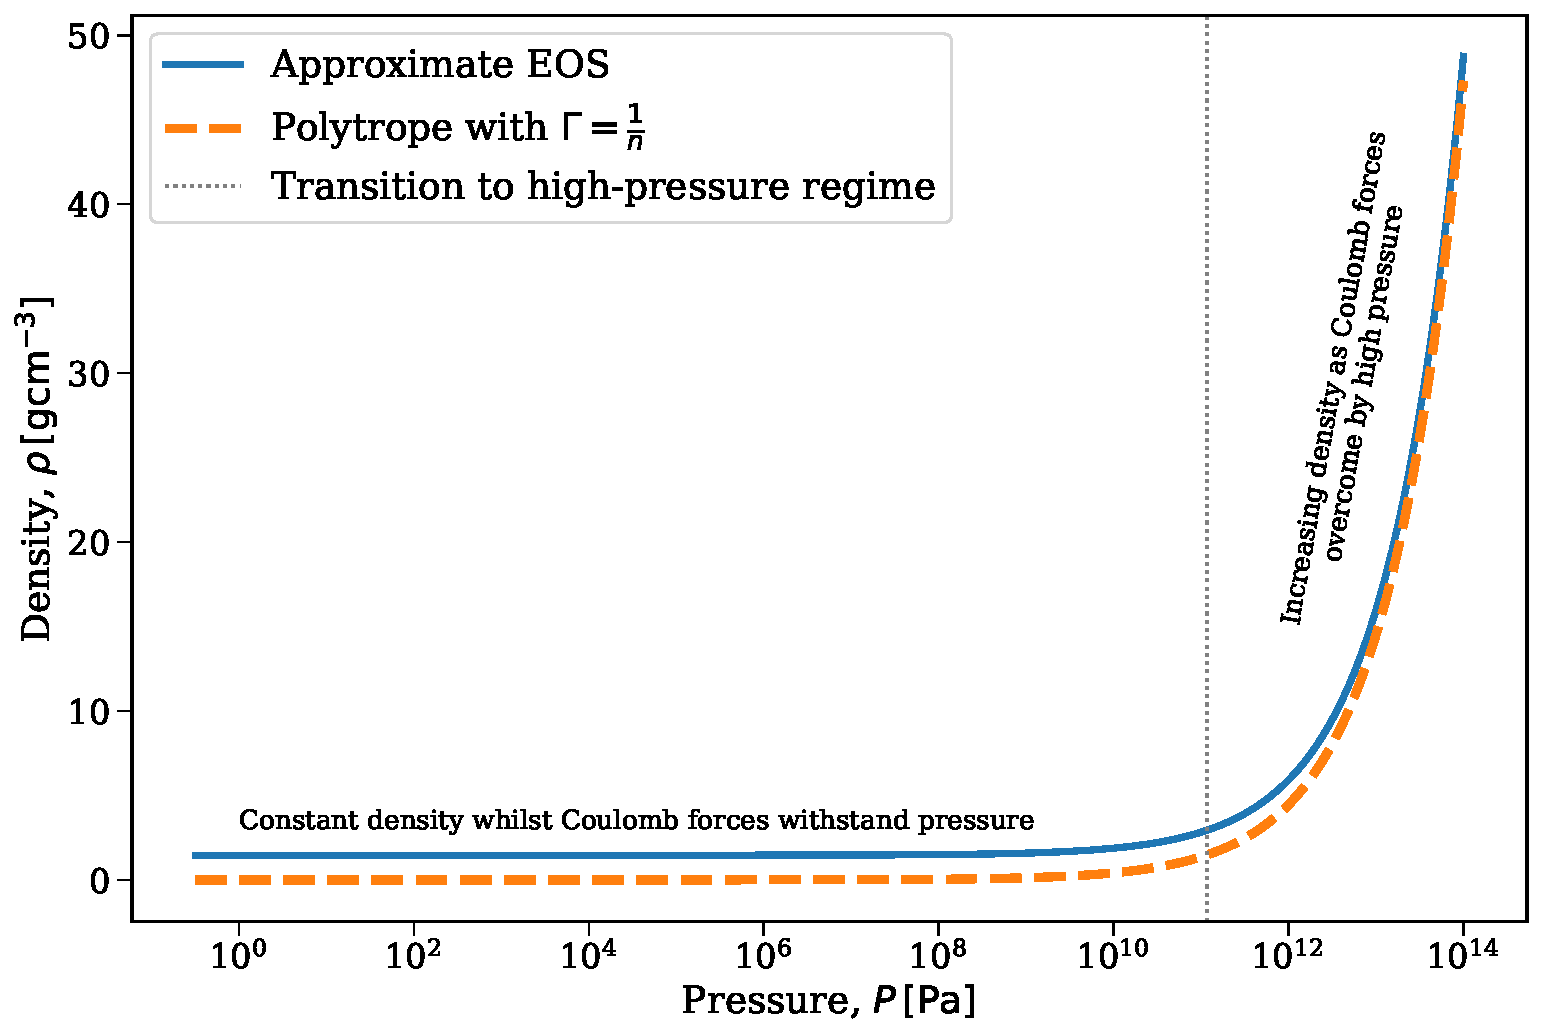
\includegraphics[width=\textwidth]{figures/2a.pdf}
    \end{center}
}

\question{2b. \textbf{Transition pressure}}
\answer{
    Just estimating by eye from the plot, the transition pressure between constant density and rising density occurs at approximately $10^{11} \unit{Pa}$. We can also verify this by finding that the density exceeds twice the initial density at a pressure of
    \begin{equation}
        \boxed{ P_{\rm trans} \approx 1.17 \times 10^{11} \unit{Pa} }
    \end{equation}
    which agrees with our initial guess. The density is constant below this transition pressure as Coulomb forces are still able to withstand the pressure at this point (such that the structure remains and the water/ice is not ``squashed''). Once the transition pressure is reached, the Coulomb forces are no longer enough to withstand the pressure and the water/ice is then slowly crushed, increasing the density.
}

\question{2c. \textbf{Temperature Assumptions}}
\answer{
    It is a good approximation that there is no temperature dependence in this equation because the degeneracy pressure plays a much more important role at these low temperatures. The water/ice is not changing phase around these temperatures and the microscopic velocities are not very high, thus the effect on the overall pressure/density is comparitively negigible.
}

\question{2d. \textbf{Maximum Mass}}
\answer{
    In order to find the maximum mass that a constant density is a good approximation, we can use the equations for the conservation of mass
    \begin{equation}
        \dv{M}{r} = 4 \pi r^2 \rho,
    \end{equation}
    and hydrostatic equilibrium
    \begin{equation}
        \dv{P}{r} = - \frac{G M}{r^2} \rho
    \end{equation}
    in the one-zone model, applying the boundary conditions that
    \begin{align}
        P_{\rm centre} &= P_{\rm trans},\quad P_{\rm edge} = 0\\
        \rho_{\rm centre} &= \rho_{\rm edge} = \rho_0\\
        r_{\rm centre} &= 0
    \end{align}
    In class we showed that for the innermost bin of the planet, the hydrostatic equilibrium equation becomes
    \begin{equation}
        P_{\rm centre} - P_{\rm edge} = \frac{2 \pi}{3} G \rho_{\rm centre}^2 r_{\rm edge}^2
    \end{equation}
    which, using the definitions of the various $P$'s and $\rho$'s, we can rearrange into
    \begin{equation}
        r_{\rm edge} = \sqrt{\frac{3}{2} \frac{P_{\rm trans}}{G \pi \rho_0^2}}
    \end{equation}
    Now we can use this in the conservation of mass equation. In this equation we find that
    \begin{align}
        \dd{M} &= M_{\rm edge} - M_{\rm centre} = M \\
        M &= 4 \pi \rho_0 r_{\rm edge}^2 (r_{\rm edge} - r_{\rm centre}) 
    \end{align}
    And therefore putting the two together gives that the maximum mass is
    \begin{equation}
        M_{\rm max} = 4 \pi \rho_0 \qty(\frac{3}{2} \frac{P_{\rm trans}}{G \pi \rho_0^2})^{\frac{3}{2}}
    \end{equation}
    which, using $P_{\rm trans} = 1.17 \times 10^{11} \unit{Pa}$ and $\rho_0 = 1.46 \unit{g}{cm^{-3}}$, gives
    \begin{equation}
        \boxed{ M_{\rm max} = 23.9 \unit{M_{\oplus}} }
    \end{equation}
    This is therefore much larger than the mass of the Earth, implying that the constant density assumption for the Earth is reasonable. I expect that the power low slope would flatten out beyond the transition pressure since the material would start to be crushed by the pressure, thus increasing less in radius for the same increase in mass.
}

\question{\textbf{Radiation-dominated star}}

\question{3a. \textbf{Temperature expression}}
\answer{
    Applying hydrostatic equilibrium, we know that
    \begin{equation}
        \frac{P_{\rm centre}}{R} \approx \frac{G M^2}{R^5}
    \end{equation}
    If we assume that $P_{\rm centre} = P_{\rm rad} = a_{\rm rad} T^4$ then we can find the expression for the temperature.
    \begin{align}
        \frac{a_{\rm rad} T^4}{R} &\approx \frac{G M^2}{R^5}\\
        \Aboxed{ T &\approx \qty(\frac{G M^2}{a_{\rm rad} R^4})^{1/4} }
    \end{align}
}

\question{3b. \textbf{Lower-limit on mass}}
\answer{
    Okay strap in folks, it's time for lots of equations! Let's set up the inequality between the radiation and gas pressure first of all (using the ideal gas law and results from part a)
    \begin{align}
        P_{\rm rad} &> P_{\rm gas} \\
        a_{\rm rad} T^4 &> n k_B T \\
        a_{\rm rad} &> n k_B T^{-3}
    \end{align}
    For the next steps we'll need to apply the expression for temperature from the first part. But this expression contains the radius and we don't want that! Never fear, we can simply write the radius in terms of density since $\rho = M / (\frac{4}{3} \pi R^3)$ (dropping factors of order unity)
    \begin{equation}
        T \approx \qty(\frac{G M^2}{a_{\rm rad}})^{1/4} \qty(\frac{M}{\rho})^{-1/3}
    \end{equation}
    Great! Now one last thing that would be useful here is to get rid of that pesky $n$ term. We could instead turn this number density into a regular density (and once again neglect factors of order unity)
    \begin{equation}
        n \approx \frac{\rho}{m_p}
    \end{equation}
    You're sitting there thinking, wait a moment Tom, you've just added $\rho$ terms which we \textit{also} don't know!? Don't worry dear reader, as for my next trick I will make them disappear (with some other fun algebra along the way!)
    \begin{align}
        a_{\rm rad} &> \frac{\rho}{m_p} k_B \qty(\frac{G M^2}{a_{\rm rad}})^{-3/4} \qty(\frac{M}{\rho}) \\
        a_{\rm rad} &> \frac{M}{m_p} k_B \qty(\frac{G M^2}{a_{\rm rad}})^{-3/4} \\
        M^{1/2} a_{\rm rad} &> \frac{k_B}{m_p} \qty(\frac{G}{a_{\rm rad}})^{-3/4} \\
        M^{1/2} &> \frac{k_B G^{-3/4}}{m_p} a_{\rm rad}^{-1/4} \\
        M &> \frac{k_B^2}{m_p^2} G^{-3/2} a_{\rm rad}^{-1/2}
    \end{align}
    What a journey it's been, now in our final step we can simply apply a definition of $a_{\rm rad}$ that we are given in the question,
    \begin{equation}
        a_{\rm rad} = \frac{k_B^4}{c^3 h^3},
    \end{equation}
    in order to get our final expression for the lower limit on the mass.
    \begin{align}
        M &> \frac{k_B^2}{m_p^2} G^{-3/2} \frac{c^{3/2} h^{3/2}}{k_B^2} \\
          &> \frac{1}{m_p^2} \qty(\frac{G}{c h})^{-3/2} \\
        \Aboxed{ M_{\rm rad} &> m_p \qty(\frac{G m_p^2}{c h})^{-3/2} }
    \end{align}
}

\question{3c. \textbf{Evaluate mass}}
\answer{
    Plugging these numbers in we find that the lower limit corresponds to
    \begin{equation}
        \boxed{ M_{\rm rad} > 29.2 \unit{M_{\odot}} }
    \end{equation}
    which is fairly close to what we would expect for radiation-dominated stars, how festive!
}

\pagebreak

\question{3d. \textbf{Polytropes}}
\answer{
    If we assume that all of the pressure in the star comes from radiation pressure then, from hydrostatic equilibrium, we have that
    \begin{align}
        \frac{P}{R} &\approx \frac{G M^2}{R^5} \\
        P &\approx G M^2 \qty(\frac{M}{\rho})^{-4/3} \\
        \implies P &\propto \rho^{4/3}
    \end{align}
    Therefore we find that $\Gamma = 4/3$ in this case and so the polytrope index is $n = 3$, like a relativistic gas, which makes sense for a radiation-dominated star! I \textit{think} the assumption we made that results in the pressure just being a function of density and not temperature is just that we are in hydrostatic equilibrium and that all of the pressure comes from radiation but I'm honestly not sure.
}

\question{3e. \textbf{Lane-Emden equation}}
\answer{
    If we could make these assumptions then we could use the Lane-Emden Equation in the same way as in lecture, specifically with $n = 3$. This would give us the density of the star as a function of the radius like in the plot in lecture 11 slide 20 and so we'd know the interal structure of stars above the radiation-dominated mass limit.
}

\end{document}

 